\documentclass{article}
\usepackage{ctex}
\usepackage{amsmath}
\usepackage{graphicx}
\usepackage{wrapfig}
\usepackage{caption}
\usepackage[top=0.8in, bottom=0.8in,left=0.8in, right=0.8in]{geometry}
\usepackage{float} 
\usepackage{subfigure}
\usepackage{subcaption}
\usepackage{bm}
\xeCJKsetup{CJKmath=true} 
\title{\textbf{第一届$\Sigma Pho$物理竞赛试题}}
\date{2023年11月}
\begin{document}
\maketitle
\newcommand \dbar {{\; \bar{} \hspace{-0.3em} \mathrm d}}
\section*{第一题、简单光学题(40分)}
\begin{itemize}
\item[(1)]一宽平行光束正入射到折射率为$n$的平凸透镜左侧平面,汇聚到平凸透镜主轴上的$F$点,已知$\overline{OF}=r_0$给出凸面型状,并给出其在直角坐标系下的标准方程,(需声明原点)。
\item[(2)]磁场透镜\par
一宽束质量,速度,电荷量分别为$m,v,q$入射到$x=0$平面。已知在第一、四象限存在大小为$B$,方向相反的磁场区域,出射后汇聚于$F(f,0)$处,给出磁场区域边界方程。
\item[(3)]电场透镜\par
一宽束质量,速度,电荷量分别为$m,v,q$入射到$x=0$平面。全空间中分布着如下电场
\[
\vec{E}=
\begin{cases}
-ky^{\alpha}\hat{y}(y>0)\\
ky^{\alpha}\hat{y}(y<0)
\end{cases}
\]
出射后汇聚于$F(f,0)$处,通过一些性质给出$\alpha$,并给出$k$的定量表达式。
\item[(4)]正经光学题\par
一束光平行于$x$轴方向入射,第一、四象限存在折射率只与$y$有关的介质,其边界是锯齿状的,使得光能垂直接着入射,出射后汇聚于$F(f,0)$处,在$(0,0)$处折射率为$n_0$,类比$(3)$给出折射率分布与边界方程.
\end{itemize}
% \clearpage

\[\]
(1)由费马原理
\[
n x \left( \theta\right) +r\left( \theta\right) =nx_{0}+r_{0}
\tag{1}
\]
由长度约束
\[
x \left( \theta \right) +r\left(\theta\right)  \cos\theta =x_{0}+r_{0}
\tag{2}
\]
$(1)-n(2)$
\[
\left( -1+n\cos \theta \right) r\left( \theta \right) =\left(n-1\right) r_{0}
\tag{3}
\]
可得
\[
r\left( \theta \right) =\dfrac{\left( n-1\right) r_{0}}{-1+n\cos \theta }
\tag{4}
\]
与极坐标下的圆锥曲线标准方程类比
\[
r=\dfrac{p}{1+e\cos \theta }
\tag{5}
\]
得
\[
e=n=\dfrac{c}{a}
\tag{6}
\]
\[
\left( n-1\right) r _{0}=\dfrac{b^{2}}{a}=\left( e^{2}-1\right) a
\tag{7}
\]
\[
a=\dfrac{r_{0}}{n+1}
\tag{8}
\]
\[
c=\dfrac{nr_{0}}{n+1}
\tag{9}
\]
\[
b=\sqrt{\dfrac{n-1}{n+1}}r_{0}
\tag{10}
\]
有
\[
\dfrac{x^{2}}{\left( \dfrac{r_{0}}{n+1}\right) ^{2}}-\dfrac{y^2}{\dfrac{n-1}{n+1}r_0^{2}}=1
\tag{11}
\]
原点在$O$右侧$\dfrac{r_0}{n+1}$
\[\]
(2)
\[r_0\cos\theta +\dfrac{mv}{qB}\sin \theta =f
\tag{12}
\]
\[
y=r\sin \theta 
\tag{13}
\]
\[
\sin \theta =\dfrac{xqB}{mv}
\tag{14}
\]
带入(12)
\[
x+r\sqrt{ {1-\left( \dfrac{xqB}{mv}\right) ^{2}}}=f
\tag{15}
\]
\[
r=\dfrac{f-x}{\sqrt{1-\left( \frac{xqB}{mv}\right) ^{2}}}
\tag{16}
\]
\[
y=\dfrac{x\left( f- x\right) }{\sqrt{\left( \frac{mv}{qB}\right) ^{2}-x^{2}}}
\tag{17}
\]
(3)
利用简谐运动周期与振幅无关的特点,可得电场力是线性恢复力
\[
\alpha =1
\tag{18}
\]
\[
-kyq=m\ddot{y}
\tag{19}
\]
\[
\omega=\sqrt{\dfrac{kq}{m}}
\tag{20}
\]
\[
t=\dfrac{T}{4}=\dfrac{\pi }{2}\sqrt{\dfrac{m}{kq}}
\tag{21}
\]
\[
\left( \dfrac{2f}{\pi v}\right) ^{2}=\dfrac{m}{kq}
\]
\[
k=\dfrac{m}{q}\left( \dfrac{\pi v}{2f}\right) ^{2}
\tag{22}
\]
(4)
类比力学中的莫培督原理与光学的费马原理
\[\delta \int p\cdot dq=0\leftrightarrow \delta \int n\cdot dl=0
\]
取$p\leftrightarrow n,q\leftrightarrow l,m=1$
\[\]
在$y$处进入电场的速度为
\[
v=n(y)
\tag{23}
\]
时间
\[
t=\dfrac{f-x}{n\left( y\right) }=\dfrac{f}{n_{0}}
\tag{24}
\]
\[
E_p=-\dfrac{1}{2}n^{2}
\tag{25}
\]
\[
\omega=\dfrac{\pi n_{0}}{2f}=\sqrt{k}
\tag{26}
\]
\[
F=-ky=-\left(\dfrac{\pi n_{0}}{2f}\right) ^{2}y
\tag{27}
\]
\[
\int F\cdot \mathrm{d}y=\dfrac{1}{2}\left( n^{2}-n(0)^2\right) =-\dfrac{1}{2}\left(\dfrac{\pi n_{0}}{2j}\right) ^{2}y^{2} 
\tag{28}
\]
\[
n=\sqrt{ n_{0}^{2}-\left(\dfrac{\pi n}{2f}\right) ^{2}y^{2}}
\tag{29}
\]
\[
x=f\left[ 1-\sqrt{1-\left( \dfrac{\pi y}{2f}\right) ^{2}}\right]
\tag{30}
\]
\textbf{评分标准:}\par
共$60$ 分\par
(1)共$9$分 $(1),(2),(3),(6),(7),(8),(9),(10),(11)$各$1$分\par
(2)共$8$分 $(12),(13),(14),(15)$各$1$分,$(16),(17)$各$2$分\par
(3)共$11$分 $(19),(20),(21),(22)$各$2$分 $(18)$$3$分\par
(4)共$12$分 $(24),(25),(26),(27),(29),(30)$各$2$分 \par

\section*{第二题、悬链线(40分)}
\begin{wrapfigure}{r}{7cm}
	\vspace{-15pt}    % 对应高度1
	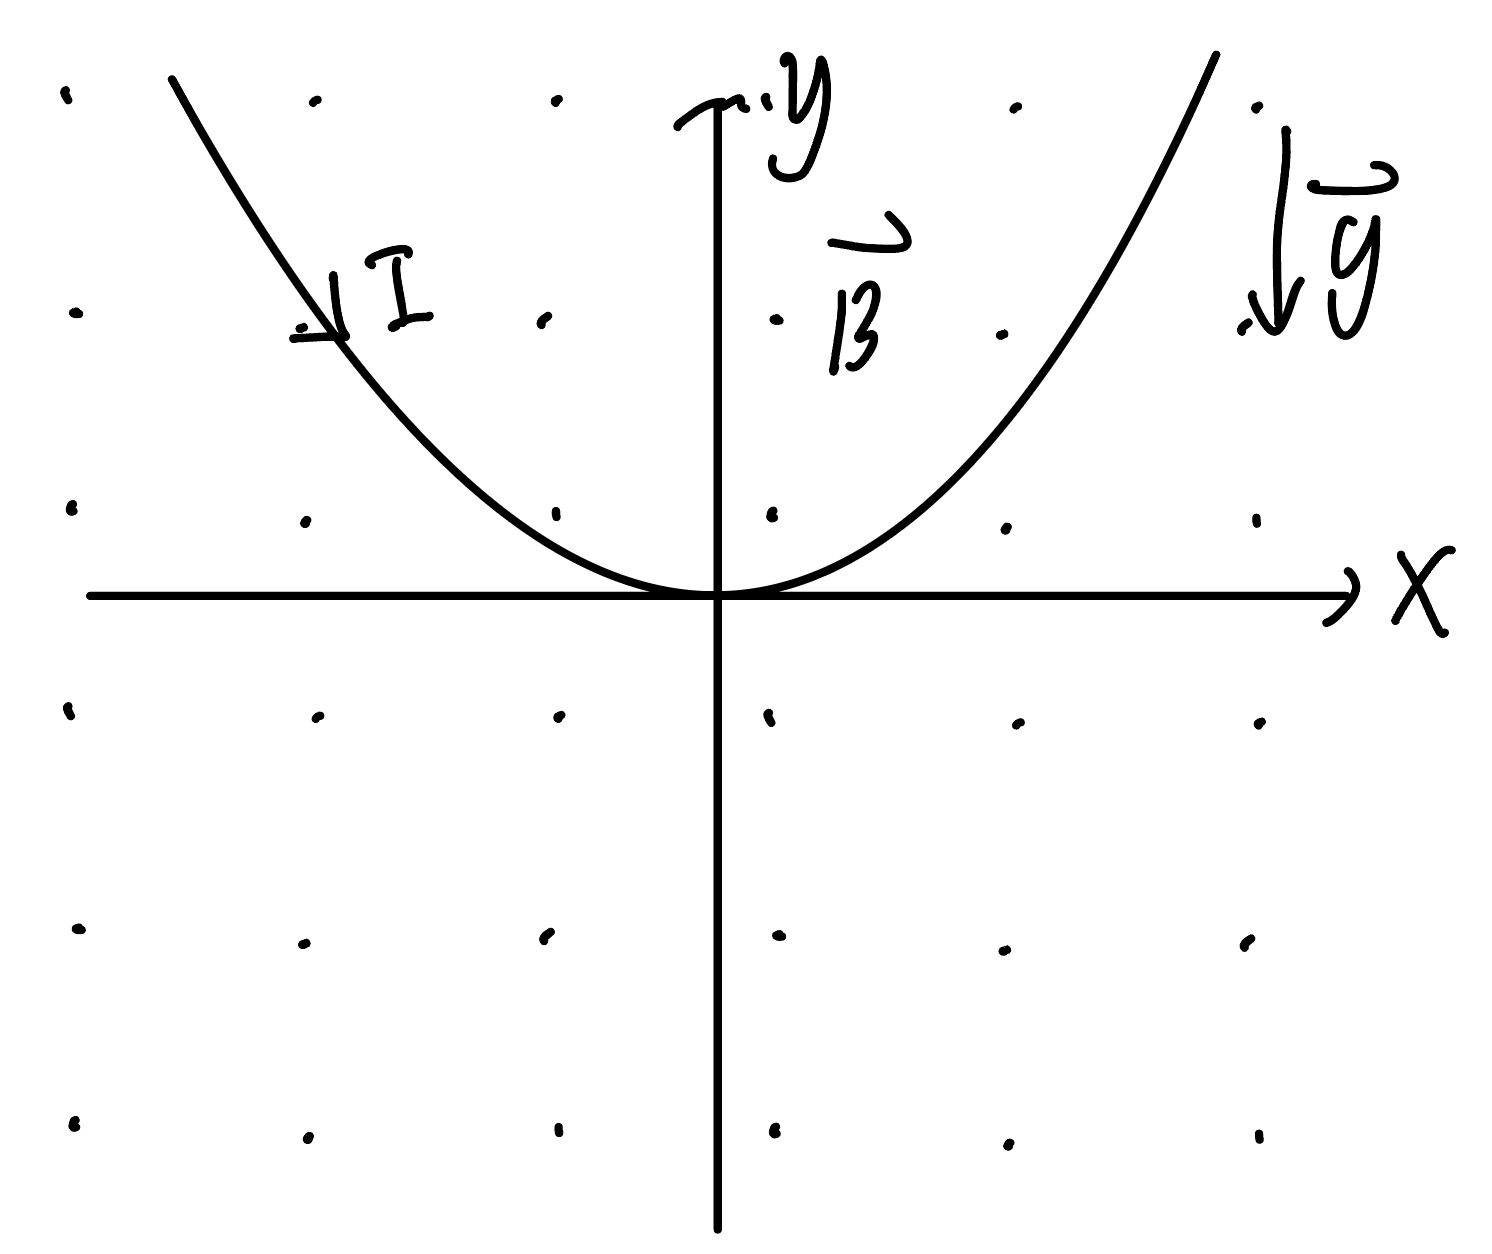
\includegraphics[width=7cm]{img/2.1.jpeg}\\
	\vspace{-15pt}    % 对应高度2
	\vspace{-15pt}    % 对应高度3
\end{wrapfigure}
竖直平面内挂有一根柔软的质量线密度为$\lambda$的均匀导线,其中通有电流$I$,存在如图所示的匀强磁场$B$,重力场$g$
已知底部$(x,y)=(0,0)$处张力为$T_0$。
试求其形状的微分方程,用$\mathrm{d}x,\mathrm{d}y$表示
\begin{itemize}
\item[(1)]取$B=0$,求其轨迹方程。\par
    注:双曲函数定义
    $$
    \cosh(x)=\dfrac{\mathrm{e}^{x}+\mathrm{e}^{-x}}{2},\sinh(\theta)=\dfrac{\mathrm{e}^{x}-\mathrm{e}^{-x}}{2}
    $$
\item[(2)]取$g=0$,求其轨迹方程。
\item[(3)]试求其形状的微分方程,用$\mathrm{d}x,\mathrm{d}y$表示.  
\end{itemize}

\[\]
(1)
\par
\begin{wrapfigure}{r}{4cm}
	\vspace{-15pt}    % 对应高度1
	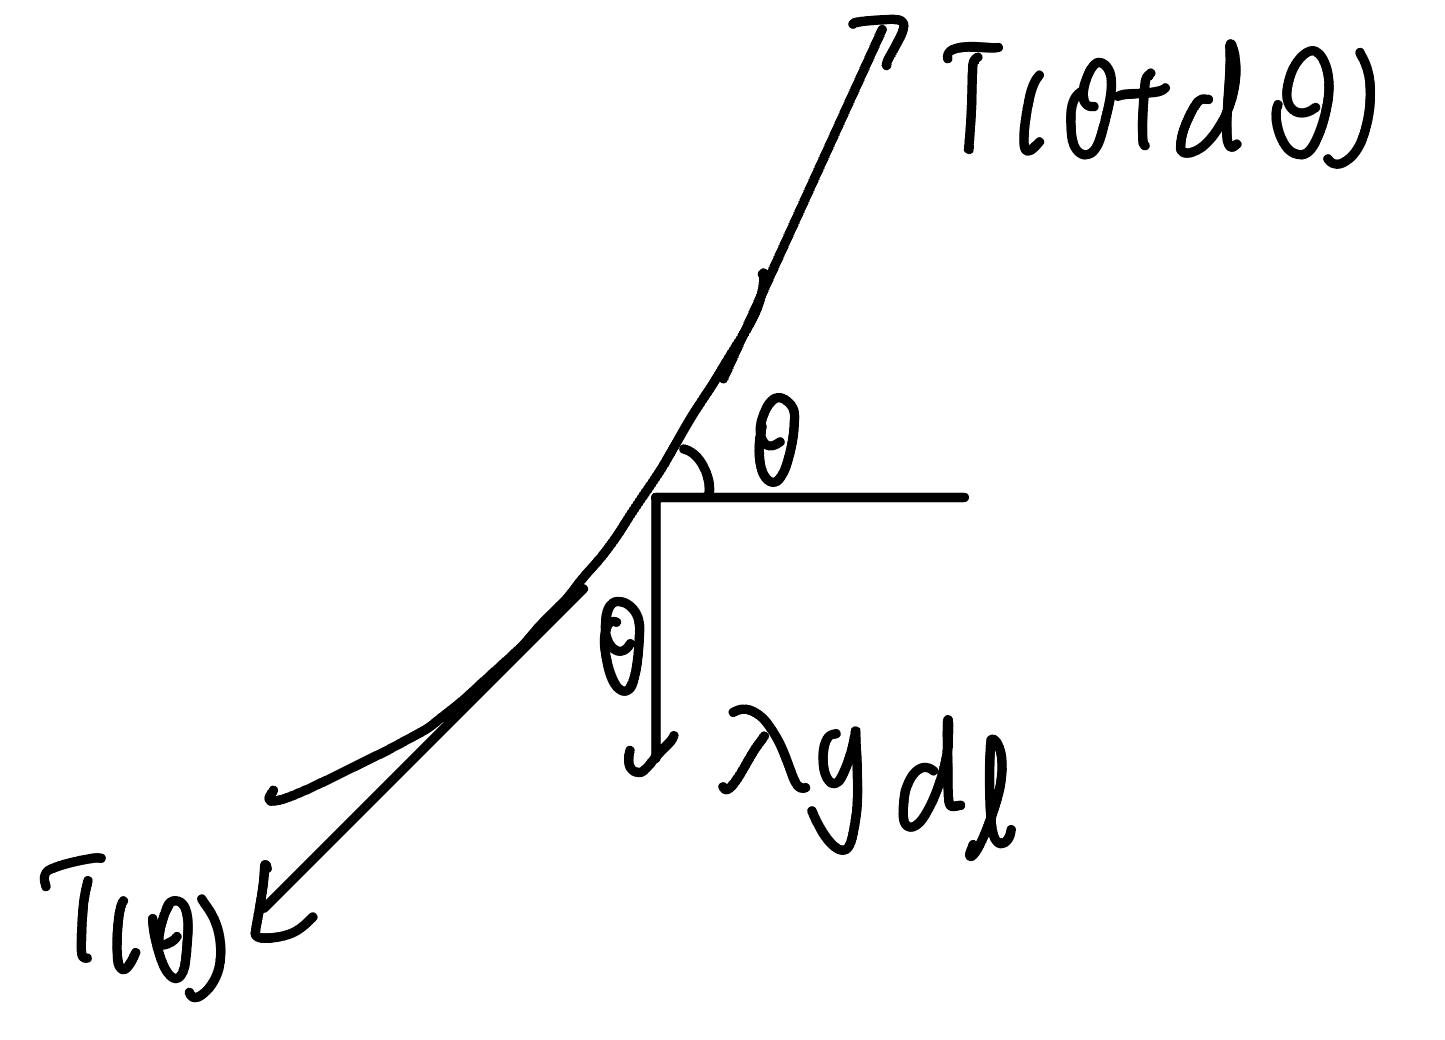
\includegraphics[width=4cm]{img/2.2.jpeg}\\
	\vspace{-15pt}    % 对应高度2
	\caption{}
	\vspace{-15pt}    % 对应高度3
\end{wrapfigure}
取微元受力分析
\[
\begin{cases}
    T\left( \theta +\mathrm{d}\theta \right) \sin \left( \theta +\mathrm{d}\theta \right) = \lambda g\mathrm{d}l+T(\theta)\sin \theta \\
    T\left( \theta +\mathrm{d}\theta \right) \cos \left( \theta +\mathrm{d}\theta \right) =T(\theta)\cos \theta 
\end{cases}
\tag{1}
\]
可得
\[
\begin{cases}
\mathrm{d}(T\sin(\theta))=\lambda g \sqrt{1+\left(\dfrac{\mathrm{d}y}{\mathrm{d}x}\right)^2}\mathrm{d}x\\
\mathrm{d}(T\cos(\theta))=0
\end{cases}
\tag{2}
\]
对(2)积分得:
\[
T\cos(\theta)=T_0
\tag{3}
\]
\[
T\sin(\theta)=T_0\dfrac{\mathrm{d}y}{\mathrm{d}x} 
\tag{4}
\]
联立(2)(4)
\[
T_{0}\dfrac{\mathrm{d}^{2}y}{\mathrm{d}x^{2}}=\lambda g\sqrt{1+\left(\dfrac{\mathrm{d}y}{\mathrm{d}x}\right)^2}
\tag{5}
\]
令$\dfrac{\mathrm{d}y}{\mathrm{d}x}=u$,得
\[
T_{0}\dfrac{\mathrm{d}u}{\mathrm{d}x}=\lambda g\sqrt{1+u^{2}}
\tag{6}
\]
\[
T_{0}\dfrac{\mathrm{d}u}{\mathrm{d}y}u=\lambda g\sqrt{1+u^{2}}
\tag{7}
\]
\[
T_{0}\dfrac{u\mathrm{d}u}{\sqrt{1+u^{2}}}=\lambda g\mathrm{d}y
\tag{8}
\]
注意到:$\mathrm{d}\left( \sqrt{1+u^{2}}\right) =\dfrac{u\mathrm{du}}{\sqrt{1+u^{2}}}$
\[
    T_0\mathrm{d}\left( \sqrt{1+u^{2}}\right) = +\lambda g\mathrm{d}y
\]
\[
    T_{0}\sqrt{1+u^{2}}-T_{0}=\lambda g\mathrm{d}y
\]
\[
    \sqrt{\left( \dfrac{T_{0}+\lambda gy}{T_{0}}\right) ^{2}-1}=\dfrac{\mathrm{d}y}{\mathrm{d}x}
\]
为了解上面的微分方程,注意到:
\[
\cosh^2 x-\sinh^2 x=1
\tag{9}
\]
令
\[
\dfrac{T_{0}+\lambda gy}{T_{0}}=\cosh \xi 
\tag{10}
\]
则上述方程化为
\[
\sinh \xi=\dfrac{\mathrm{d}y}{\mathrm{d}x}
\tag{11}
\]
对(10)求导
\[
\dfrac{\lambda g}{T_{0}}=\sinh \xi\dfrac{\mathrm{d}\xi}{\mathrm{d}y}
\tag{12}
\]
带入(11)
\[
\dfrac{\lambda g}{T_{0}}\dfrac{\mathrm{d}y}{\mathrm{d}\xi}=\dfrac{\mathrm{d}y}{\mathrm{d}x}
\tag{13}
\]
得到
\[
\xi=\dfrac{\lambda g}{T_{0}} x
\tag{14}
\]
可得
\[
y=\dfrac{T_0\left(\cosh\left(\dfrac{\lambda g}{T_{0}} x\right)-1\right)}{\lambda g}
\tag{15}
\]
(2)
\par
\begin{wrapfigure}{r}{4cm}
	\vspace{-15pt}    % 对应高度1
	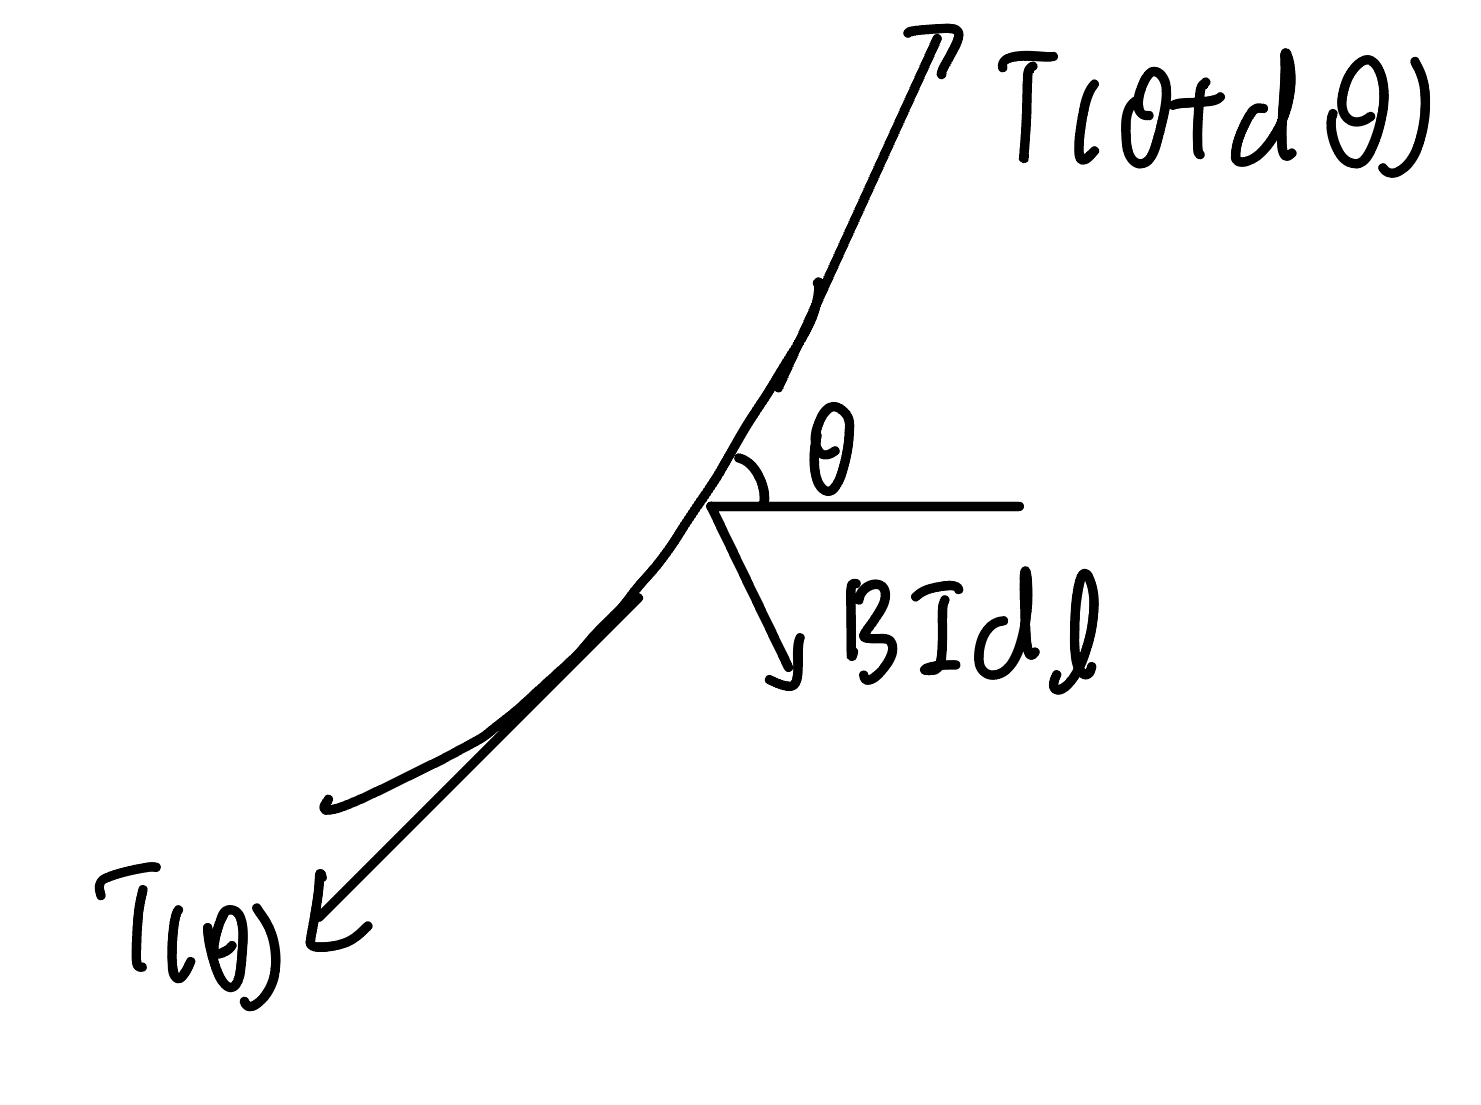
\includegraphics[width=4cm]{img/2.3.jpeg}\\
	\vspace{-15pt}    % 对应高度2
	\caption{}
	\vspace{-15pt}    % 对应高度3
\end{wrapfigure}
取微元受力分析,可得起沿着径向,有
\[
2T_0\frac{1}{2}\mathrm{d}=BI\mathrm{d}l
\tag{16}
\]
可得
\[
R=\dfrac{T_0}{BI}
\tag{17}
\]
可得方程
\[
x^2+\left(y-\dfrac{T_0}{BI}\right)^2=\left(\dfrac{T_0}{BI}\right)^2
\tag{18}
\]
(3)
\par
\begin{wrapfigure}{r}{4cm}
	\vspace{-15pt}    % 对应高度1
	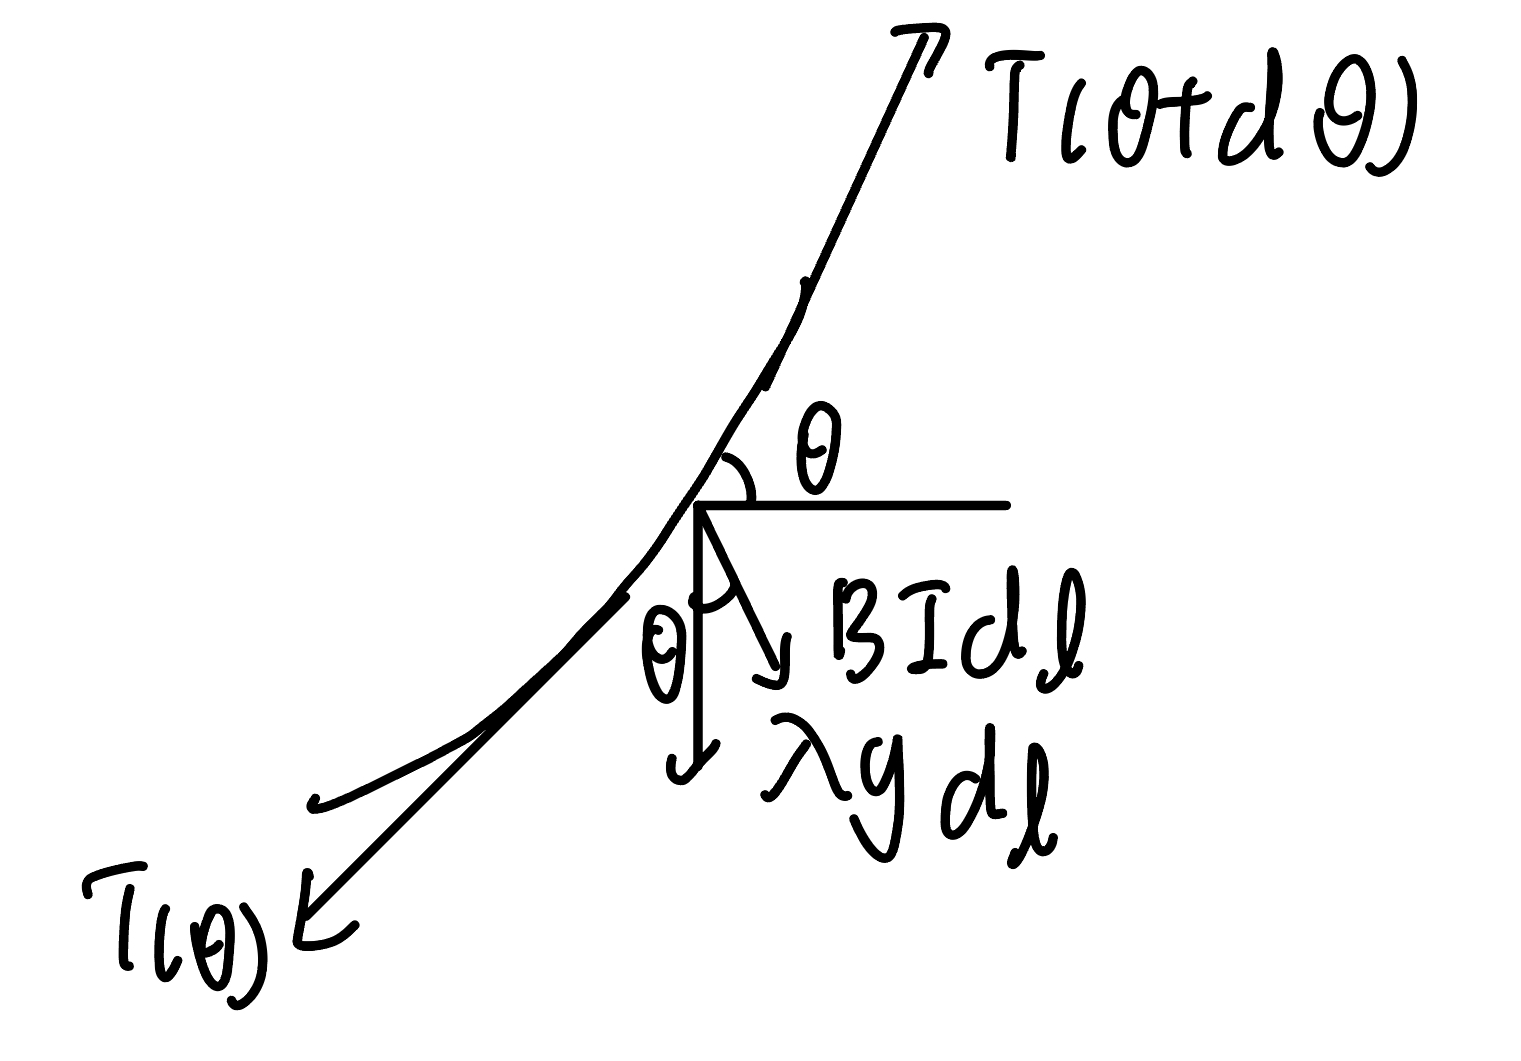
\includegraphics[width=4cm]{img/2.4.jpeg}\\
	\vspace{-15pt}    % 对应高度2
	\caption{}
	\vspace{-15pt}    % 对应高度3
\end{wrapfigure}
取微元受力分析
\[
\begin{cases}
    T\left( \theta +\mathrm{d}\theta \right) \sin \left( \theta +\mathrm{d}\theta \right) =BI\mathrm{d}l\cos \theta +\lambda g\mathrm{d}l+T(\theta)\sin \theta \\
    T\left( \theta +\mathrm{d}\theta \right) \cos \left( \theta +\mathrm{d}\theta \right) +BI\mathrm{d}l\sin \theta =T(\theta)\cos \theta 
\end{cases}
\tag{19}
\]
可得
\[
\begin{cases}
\mathrm{d}(T\sin(\theta))=BI\mathrm{d}x+\lambda g \sqrt{1+\left(\dfrac{\mathrm{d}y}{\mathrm{d}x}\right)^2}\mathrm{d}x\\
\mathrm{d}(T\cos(\theta))-BI\mathrm{d}y
\end{cases}
\tag{20}
\]
对(20)积分得:
\[
T\cos(\theta)=T_0-BIy
\tag{21}
\]
\[
T\sin(\theta)=(T_0-BIy)\dfrac{\mathrm{d}y}{\mathrm{d}x} 
\tag{22}
\]
联立(20)(22)
\[
T_{0}\dfrac{\mathrm{d}^{2}y}{\mathrm{d}x^{2}}-BI\left( \dfrac{\mathrm{d}y}{\mathrm{d}x}\right) ^{2}-BIy\dfrac{\mathrm{d}^{2}y}{\mathrm{d}x^{2}}=BI+\lambda g\sqrt{1+\left(\dfrac{\mathrm{d}y}{\mathrm{d}x}\right)^2}
\tag{23}
\]
令$\dfrac{\mathrm{d}y}{\mathrm{d}x}=u$,得
\[
T_{0}\dfrac{\mathrm{d}u}{\mathrm{d}x}-BIu^{2}-BIy\dfrac{\mathrm{d}u}{\mathrm{d}x}=BI+\lambda g\sqrt{1+u^{2}}
\tag{24}
\]
\[
T_{0}\dfrac{\mathrm{d}u}{\mathrm{d}y}u=BI\left(1+u^{2}\right)+BIyu\dfrac{\mathrm{d}u}{\mathrm{d}x}+\lambda g\sqrt{1+u^{2}}
\tag{25}
\]
\[
T_{0}\dfrac{u\mathrm{d}u}{\sqrt{1+u^{2}}}=BI\sqrt{1+u^{2}}\mathrm{d}y+BIy\dfrac{u\mathrm{d}u}{\sqrt{1+u^{2}}}+\lambda g\mathrm{d}y
\tag{26}
\]
注意到:$\mathrm{d}\left( \sqrt{1+u^{2}}\right) =\dfrac{u\mathrm{du}}{\sqrt{1+u^{2}}}$
\[
    T_0\mathrm{d}\left( \sqrt{1+u^{2}}\right) =BI\mathrm{d}\left( y\sqrt{1+u^{2}}\right) +\lambda g\mathrm{d}y
\tag{27}
\]
\[
    T_{0}\sqrt{1+u^{2}}-T_{0}=BI\mathrm{d}\left( y\sqrt{1+n^{2}}\right) +\lambda g\mathrm{d}y
    \tag{28}
\]
\[
    \sqrt{\left( \dfrac{T_{0}+\lambda gy}{T_{0}-BIy}\right) ^{2}-1}=\dfrac{\mathrm{d}y}{\mathrm{d}x}
    \tag{29}
\]
\textbf{评分标准:}\par
共$40$ 分\par
(1)共$15$分 $(1),(2),(3),(4),(5),(6),(7),(8),(9),(10),(11),(12),(13),(14),(15)$各$1$分\par
(2)共$5$分 $(16)$各$1$分,$(17),(18)$各$2$分\par
(3)共$20$分 $(19),(20),(21),(22),(23),(24),(25),(26),(27),(28),(29),(30),(31),(32),(33)$各$2$分\par

\section*{第三题、液体表面张力系数的确定(40分)}
众所周知液体有表面张力,但是往往表面张力系数是由实验测定的,下尝试通过理论方式建立。\par
\begin{itemize}
\item[(1)]已知热力学第一定律的微分形式是$\mathrm{d}U=Y\mathrm{d}y+T\mathrm{d}s$,其中$Y$是广义力,$y$是广义坐标,给出表面张力系统的热力学第一定律的微分形式。
\end{itemize}\par
液体内部的分子,其周围所受的力在平均后是各向同性的,但在液体表面,由于上面部分没有液体分子。用“作用力球”来说明,就是液体内部“作用力球”完整,而在表面“作用力球”少了一个球冠,从而导致了其受力并不为零,下给出定量分析的模型。\par
计液体内任意两个相邻的分子之间的相互作用能为$\varepsilon$,且液体内部一个分子与$n$个分子相邻,在表面与$\zeta n$个分子相邻.
\begin{itemize}
\item[(2)]给出内外分子势能的差值。
\item[(3)]设表面的粒子面密度为$\sigma_n$,求形成$\mathrm{d}A_S$面积的表面时做的功,并用$\sigma_n,\varepsilon,n,\zeta$表示表面张力系数$\sigma$。\par
\end{itemize}
\par
下确定$\varepsilon$.考虑液体汽化过程,给出摩尔汽化热$L_m$(认为是从内部分子汽化出去的).
\begin{itemize}
\item[(4)]给出$\varepsilon$,用$L_m,N_A,n$表示表面张力系数。
\item[(5)]认为一个分子占据半径为$d$的空间,给出液体分子的摩尔质量$\mu$和密度$\rho$,用$\zeta,L_m,N_A,\rho,\mu$表示表面张力系数$\sigma$ 
\end{itemize}
\par
现考虑混合液体的表面张力系数,设液体的两种组分为$\mu_1,\rho_1,d_1,n_1,\zeta_1,\sigma_{n_1}$和$\mu_2,\rho_2,d_2,n_2,\zeta_2,\sigma_{n_2}$,其中$n$数密度,液体内两种组分每个分子与均与$x_1,x_2$个分子相邻。两种组分之间的相互作用能为$\varepsilon_{11},\varepsilon_{22},\varepsilon_{12}$,并假设$|\varepsilon_{12}|=\sqrt{|\varepsilon_{11}||\varepsilon_{22}|}$
\begin{itemize}
\item[(6)]给出混合液体的表面张力系数$\sigma_{12}$,用$\mu_1,\rho_1,d_1,n_1,\zeta_1,\sigma_{n_1},x_1,\mu_2,\rho_2,d_2,n_2,\zeta_2,\sigma_{n_2},x_2$
\end{itemize}

\[\]
(1)由表面张力公式
\[F=l\sigma\tag{1}\]
表面张力作功
\[\dbar W=F\cdot \mathrm{d}x=\sigma\mathrm{d}A\tag{2}\]
\[\mathrm{d}A=l\mathrm{d}x\tag{3}\]
代入可得
\[\mathrm{d}U=\sigma\mathrm{d}S+T\mathrm{d}S\tag{4}\]
(2)由题意
\[
\Delta U=(1-\zeta)\dfrac{-\varepsilon}{2}n
\tag{5}\]
(3)由题意
\[
\dbar W=\sigma_n\mathrm{d}A_S(1-\zeta)\dfrac{- \varepsilon}{2}n
\tag{6}\]
(4)由题意
\[
-\dfrac{n}{2}\varepsilon N_A=L_m
\tag{7}\]
\[
\varepsilon=\dfrac{-2L_m}{nN_A}
\tag{8}\]
(5)
\[
d^3N_A=\dfrac{\mu}{\rho}
\tag{9}\]
\[
d=\left(\dfrac{\mu}{\rho N_A}\right)^{\frac{1}{3}}
\tag{10}\]
\[
\sigma=(1-\zeta)\dfrac{L_m}{N_A}\left(\dfrac{\rho N_A}{\mu}\right)^{\frac{3}{2}}
\tag{11}\]
(6)类似于上面的方法
\[
\Delta U_1=(1-\zeta_1)x_1\dfrac{n_1}{n_1+n_2}\dfrac{-\varepsilon_{11}}{2}+(1-\zeta_1)x_1\dfrac{n_2}{n_1+n_2}\dfrac{-\varepsilon_{12}}{2}
\tag{12}\]
\[
\Delta U_2=(1-\zeta_2)x_1\dfrac{n_1}{n_1+n_2}\dfrac{-\varepsilon_{12}}{2}+(1-\zeta_1)x_1\dfrac{n_2}{n_1+n_2}\dfrac{-\varepsilon_{22}}{2}
\tag{13}\]
\[
\dbar W=\sigma_{n_1}\mathrm{d} A_S \Delta U_1+\sigma_{n_2}\mathrm{d} A_S \Delta U_2=\sigma_{12}\mathrm{d} A_S
\tag{14}\]
\[
\begin{aligned}
\sigma_{12}=\left[(1-\zeta_1)x_1\dfrac{n_1}{n_1+n_2}\dfrac{-\varepsilon_{11}}{2}+(1-\zeta_1)x_1\dfrac{n_2}{n_1+n_2}\dfrac{-\sqrt{\varepsilon_{11}\varepsilon_{22}}}{2}\right]\sigma_{n_1}\\
+\left[(1-\zeta_2)x_1\dfrac{n_1}{n_1+n_2}\dfrac{-\sqrt{\varepsilon_{11}\varepsilon_{22}}}{2}+(1-\zeta_1)x_1\dfrac{n_2}{n_1+n_2}\dfrac{-\varepsilon_{22}}{2}\right]\sigma_{n_2}
\end{aligned}
\tag{15}\]

\textbf{评分标准:}\par
共$40$ 分\par
(1)共$7$分 $(1),(3)$各$1$分,$(2)$$2$分,$(4)$$3$分\par
(2)共$3$分 $(5)$$3$分\par
(3)共$3$分 $(6)$$3$分\par
(4)共$6$分 $(7),(8)$各$3$分\par
(5)共$9$分 $(9),(10),(11)$各$3$分\par
(5)共$12$分$(12),(13),(14),(15)$各$4$分

\section*{第四题、受限三体问题与拉格朗日点(60分)}
	对于任意给定的$m_1,m_2,m_3$,仅在万有引力的作用下运动,在任意给定初值的条件下求解$m_1,m_2,m_3$的运动的问题称作三体问题,时至今日依旧没有解析解,但对于$m_1,m_2\gg m$的情况下,且完全忽略$m$对$m_1,m_2$运动的影响,称为受限三体问题。\par
	在这类问题中,有一些点满足在$m_1,m_2$公转系中静止的条件,这些点称为拉格朗日点。\par
	下认为$m_1,m_2$均作圆周运动,以质心为原点,$(r_1,0)$表示$m_1$的位置,$(-r_2,0)$表示$m_2$的位置,且$r=r_1+r_2$。\par
\begin{itemize}
\item[(1)]	给出任意$(x,y)$处的有效势.(单位质量势能,$m_1,m_2$除外)
\item[(2)]	给出拉格朗日点满足的方程(无需求解)给出$y=0$拉格朗日点的个数,并定性描述其位置.\par
在一定近似下,我们可以求解,如令
$$\varepsilon=\dfrac{m_1}{m_2}\to 0.$$
\item[(3)]	给出$y=0$时的零阶解,并进一步描述位置.
\item[(4)]	给出$y=0$时的一阶解,并给出坐标.
\item[(5)]	求出剩下的点,并指出其特殊几何关系.
\end{itemize}

\[\]
(1)
先求公转角速度
\[
\dfrac{Gm_1 m_2}{r^2}=\Omega^2 r_1 m_1=\Omega^2 \dfrac{m_1 m_2 r}{m_1 +m_2}
\]
\[
=>\Omega^2=\dfrac{G(m_1+m_2)}{r^3}\tag{1}
\]
\[
V_{\mathbf{eff}}(x,y)=
\dfrac{-Gm_1}{\sqrt{(x-r_1)^2+y^2}}
-\dfrac{Gm_2}{(\sqrt{(x+r_2)^2+y^2}}
-\dfrac{1}{2}\dfrac{G(m_1+m_2)}{r^3}(x^2+y^2)\tag{2}
\]
(2)
\[
\dfrac{\partial V_{\mathbf{eff}}}{\partial x}
=0
=\dfrac{Gm_1(x-r_1)}{[(x-r_1)^2+y^{2}]^{\frac{3}{2}}}
+\dfrac{Gm_2(x+r_2)}{[(x+r_2)^2+y^{2}]^{\frac{3}{2}}}
-\dfrac{G(m_1+m_2)}{r^3}x
\tag{3}
\]
\[
\dfrac{\partial V_{\mathbf{eff}}}{\partial y}=0
=\dfrac{Gm_1 y}{[(x-r_1)^2+y^{2}]^{\frac{3}{2}}}
+\dfrac{Gm_2 y}{[(x+r_2)^2+y^{2}]^{\frac{3}{2}}}
-\dfrac{G(m_1+m_2)}{r^3}y
\tag{4}
\]
对于$y=0,(4)$易知满足,对于$(3)$,同除$\dfrac{G(m_1+m_2)}{r}$,得
\[
 \dfrac{r_2(x-r_1)}{|x-r_1|^3}
+\dfrac{r_2(x+r_2)}{|x+r_2|^3}
=\dfrac{x}{r^2}\tag{3'}
\]
令$f(x)=\dfrac{r_2(x-r_1)}{|x-r_1|^3}+\dfrac{r_2(x+r_2)}{|x+r_2|^3}$,有
\[
\lim_{x \to -\infty}f(x)=0^-\tag{5}
\]
\[
\lim_{x \to (-r_2)^-}f(x)=-\infty,\lim_{x \to (-r_2)^+}f(x)=+\infty\tag{6}
\]
\[
\lim_{x \to (r_1)^-}f(x)=-\infty,\lim_{x \to (r_1)^+}f(x)=+\infty\tag{7}
\]
\[
\lim_{x \to +\infty}f(x)=0^+\tag{8}
\]
\[可见,有3根\tag{9}\]
\[L_1(-\infty,-r_2),L_2(-r_2,r_1),L_3(r_1,\infty)\tag{10}\]
(3)
在$\dfrac{m_2}{m_1}=\varepsilon\to 0$
\[
r_1=\dfrac{m_2}{m_1+m_2}r=\dfrac{\varepsilon}{\varepsilon+1}r\approx \varepsilon(1-\varepsilon)r\tag{11}
\]
\[
r_2=\dfrac{m_1}{m_1+m_2}r=\dfrac{1}{\varepsilon+1}r\approx (1-\varepsilon)r\tag{12}
\]
保留零阶,代入$(4)$式
\[
\dfrac{rx}{|x|^3}=\dfrac{x}{r^2}\tag{13}
\]
\[
=>x=\pm r\tag{14}
\]
\[
可得L_1,L_2在m_2附近,L_3在离原点r附近\tag{15}
\]
(4)
对于$L_1,L_2$,令$x=-r+\delta_{1,2}r$,带入$(4)$式,保留一阶
\[
-\dfrac{(1-\varepsilon)r}{(-r+\delta_{1,2}r-\varepsilon r)^2}
\pm 
\dfrac{\varepsilon r}{(-r + \delta_{1,2} r +(1-\varepsilon)r)^2}=\dfrac{-r+\delta_{1,2}r}{r^2}\tag{16}
\]
\[
\pm \dfrac{\varepsilon}{(\delta_{1,2}-\varepsilon)^2}=3(\delta_{1,2}-\varepsilon)
\]
由于两边小量阶数一致,取$1\gg\delta_{1,2}\gg\varepsilon$ ,带入有
\[
\pm \dfrac{\varepsilon}{\delta_{1,2}^2}\left(1+\dfrac{2\varepsilon}{\delta_{1,2}}\right)=3(\delta_{1,2}-\varepsilon)
\]
\[
=>\pm  \dfrac{\varepsilon}{\delta_{1,2}^2}=3 \delta_{1,2}^2
\]
\[
=>\delta_{1,2}= \pm \left(\dfrac{\varepsilon}{3}\right)^{\frac{1}{3}}\tag{17}
\]
对于$L_3$,令$x=r+\delta_3$
\[
\dfrac{1-\varepsilon}{(1+\delta_3-\varepsilon)^2}+\dfrac{\varepsilon}{(1+\delta_3+1-\varepsilon)^2}=1+\delta_3\tag{18}
\]
得
\[
\delta_3=\dfrac{5}{12}\varepsilon\tag{19}
\]
故
\[
L_1\left(-r-(\dfrac{\varepsilon}{3})^{\frac{1}{3}}r,0\right)\tag{20}
\]
\[
L_2\left(-r+(\dfrac{\varepsilon}{3})^{\frac{1}{3}}r,0\right)\tag{21}
\]
\[
L_3\left(r+\dfrac{5}{12}\varepsilon r,0\right)\tag{22}
\]
(5)
由$(4)\times \dfrac{x}{y}$与$(3)$相减得
\[
\dfrac{-r_1 r_2}{[(r_1-x)^2+y^2]^{\frac{2}{3}}}
+\dfrac{r_1 r_2}{[(r_2+x)^2+y^2]^{\frac{2}{3}}}
=0\tag{23}
\]
由$(4)\times \dfrac{1}{y}$得
\[
\dfrac{r_2}{[(r_1-x)^2+y^2]^{\frac{2}{3}}}
+\dfrac{r_1}{[(r_2+x)^2+y^2]^{\frac{2}{3}}}
=\dfrac{1}{r^2}\tag{24}
\]
$(23),(24)$可看作关于分母的一元二次方程组,解得
\[
(r_1-x)^2+y^2=(r_2+x)^2+y^2=r^2\tag{25}
\]
\[
x=\dfrac{r_1-r_2}{2},y=\pm\dfrac{\sqrt{3}r}{2}\tag{26}
\]
\[
可得L_4,L_5与 m_1,m_2构成两个等边三角形\tag{27}
\]
\textbf{评分标准:}\par
共$60$ 分\par
(1)共$4$分 $(1),(2)$各$2$分\par
(2)共$16$分 $(3),(4)$各$2$分,$(5),(6),(7),(8)$各$2$分 $(9)$各$2$ $(10)$$2$分\par
(3)共$8$分 $(11),(12),(13)$各$1$分 $(14)$$3$分 $(15)$ $2$分\par
(4)共$20$分 $(16)$$2$分 $(17)$ $6$分 $(18)$$2$分 $(19)$各$4$分 $(20),(21),(22)$各$2$分\par
(5)共$12$分 $(23)$ $2$分 $(25)$ $4$分 $(26)$ $4$分 $(27)$ $2$分\par

\section*{第五题、匀强磁场中带电小球在圆盘上的运动(50分)}
\begin{wrapfigure}{r}{7cm}
	\vspace{-15pt}    % 对应高度1
	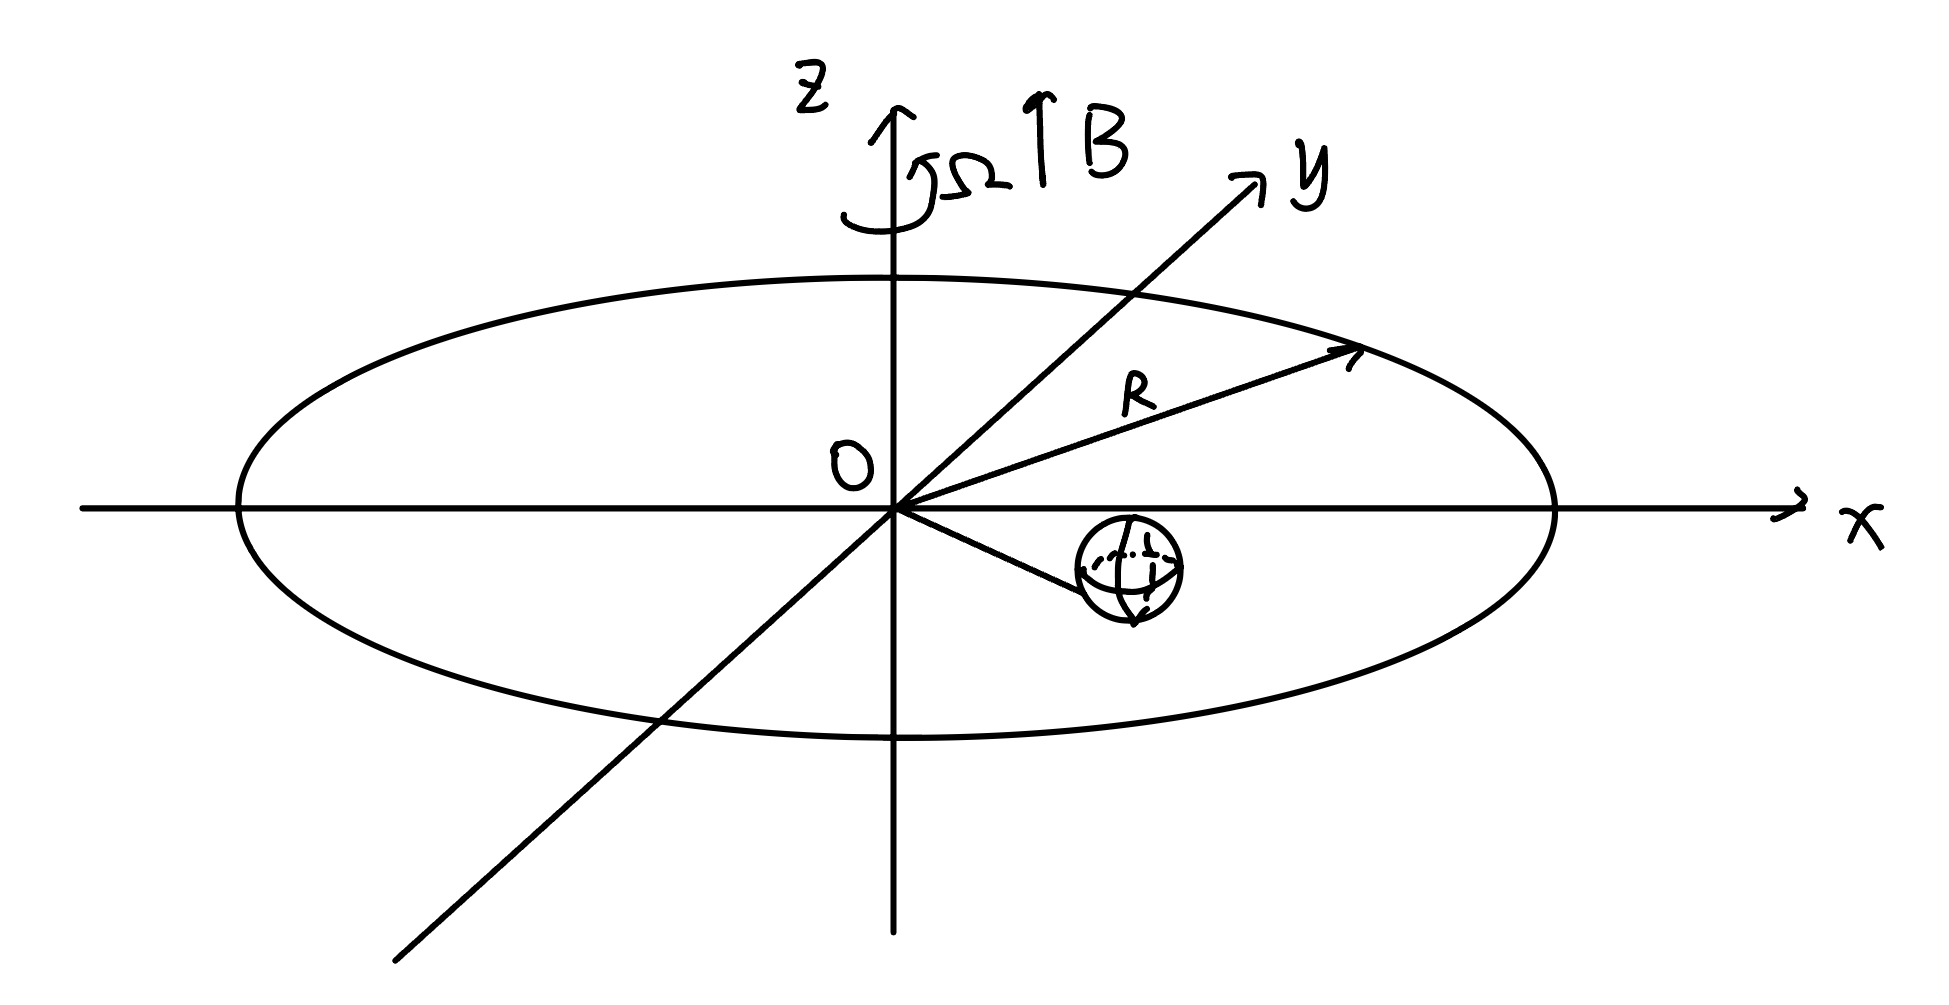
\includegraphics[width=7cm]{img/5.1.jpeg}\\
	\vspace{-15pt}    % 对应高度2
	\vspace{-15pt}    % 对应高度3
\end{wrapfigure}
考虑一个沿$z$轴以匀角速度$\Omega$转动的薄圆盘半径为$R$,质量为$M$。有一半径为$r$,均匀带电量为$Q$,质量为$m$的小球,小球与圆盘间无滑动。全空间存在竖直向上的匀强磁场,大小为$B$.\par
初始将小球静止放在$(r_0,0,0)$处,考虑其运动。\par
\begin{itemize}
\item[(1)]当带电小球以$\vec{\omega}$转动时,求带电小球的总磁矩$\vec{\mu}$。\par
注:磁矩定义$\vec{\mu}=I\vec{S}$\par
\item[(2)]初始$t=0$,求解之后的运动。
\end{itemize}

\[\]
(1)解:按定义
\[\vec{\mu }=\dfrac{1}{2}\int \rho \vec{r}\times \vec{v}dV\tag{1}\]
\[Q=\dfrac{4}{3}\pi R^{3}\rho\tag{2}\]
得
\[\vec{\mu }=\dfrac{1}{5}Q\vec{w}r^{2}\tag{3}\]
(2)解:由无相对滑动,故$\omega_z=0$
\[\vec{v_{c}}+\left( -r\hat{z}\right) \times \vec{w}=\left( x\hat{x}+y\hat{y}\right) \times \left( \Omega \hat{z}\right) \tag{4}\]
\[
\begin{cases}
    \dot{x}-\omega_{y}r=-\Omega y\\
    \dot{y}+\omega_{x} r=\Omega x
\end{cases}
\tag{5}
\]
质心运动定理
\[
F_x \hat{x}+F_y\hat{y}+Q\vec{v}_{c}\times \left( B\hat{z}\right) =m\left( \ddot{x}\hat{x}+ \ddot{y}\hat{y}\right)
\tag{7}
\]
质心转动定理
\[
\dfrac{2}{5}mr^{2}\dfrac{\mathrm{d}\vec{\omega}}{\mathrm{d}t}=\left( -r\right) \hat{z}\times \left( F_{x}\hat{x}+F_{y}\hat{y}\right) +\vec{\mu }\times \vec{B}
\tag{8}
\]
\[
\begin{cases}
    rF_y+\mu _{y}B=\dfrac{2}{5}mr^{2}\dot{\omega_x}\\
    -\left( rF_{x}+\mu _{x}B\right) =\dfrac{2}{5}mr^{2}\dot{\omega_y}
\end{cases}
\tag{9}
\]
消去$F_z,F_y,\omega_x,\omega_y$,得二阶二元线性微分方程组
\[
\begin{cases}
    \dfrac{7}{5}mr\ddot{y}+\left( \dfrac{6}{5}QBr-\dfrac{2}{5}mr\Omega \right) \dot{x}+\dfrac{1}{5}QrB\Omega y=0\\
    \dfrac{7}{5}mr\ddot{x}-\left( \dfrac{6}{5}QBr-\dfrac{2}{5}mr\Omega \right) \dot{y}+\dfrac{1}{5}QrB\Omega x=0
\end{cases}
\tag{10}
\]
令$\tilde{\xi}=x+\i y$,将(10)式中两式相加,得
\[
\dfrac{7}{5}mr\ddot{\tilde{\xi}}+\left( \dfrac{6}{5}QBr-\dfrac{2}{5}mr\Omega \right)\dot{\tilde{\xi}}\i+\dfrac{1}{5}QB\Omega r\tilde{\xi}=0
\tag{11}
\]
令$\tilde{\xi}=e^{\i\omega t}$,带入(11)式
\[
-\dfrac{7}{5}mr\omega ^{2}-\left( \dfrac{6}{5}QBr -\dfrac{2}{5}mr\Omega \right) \omega +\dfrac{1}{5}QB\Omega r=0
\tag{12}
\]
得
\[
\omega_{1}=\dfrac{3QBr-mr\Omega +\sqrt{\left( 3QBr-mr\Omega \right) ^{2}+7mr^{2}\omega^{2}QB\Omega }}{-7mr}
\tag{13}
\]
\[
\omega_{2}=\dfrac{3QBr-mr\Omega -\sqrt{\left( 3QBr-mr\Omega \right) ^{2}+7mr^{2}\omega^{2}QB\Omega }}{-7mr}
\tag{14}
\]
将两解线性叠加,并重新拆分为$x,y$,有
\[
x=A\cos \left( \omega _{1}t\right) +B\cos\left( \omega_{2}t\right)
\]
\[
y=A\sin \left( \omega _{1}t\right) +B\sin\left( \omega_{2}t\right)
\]
带入初值
\[
\begin{cases}
    A+B=r_0\\
    A\omega _{1}+A\omega _{w}=\Omega r_{0}
\end{cases}
\tag{15}
\]
解得
\[
\begin{cases}
A=-\dfrac{r_{0}\left( \omega _{2}-\Omega \right) }{\omega _{1}-\omega _{2}}\\
B=\dfrac{r_{0}\left( \omega _{1}-\Omega \right) }{\omega _{1}-\omega _{1}}
\end{cases}
\tag{16}
\]
\textbf{评分标准:}\par
共$50$ 分\par
(1)共$5$分 $(2)$各$1$分,$(1),(3)$各$2$分\par
(2)共$45$分 $(4),(6)$各$2$分,$(8),(12),(13),(14),(15),(16)$各$3$分,$(5),(7),(9),(10),(11)$$4$分,指出$\omega_z=0$给$3$分\par

\section*{第六题、Arago圆盘(40分)}
\begin{wrapfigure}{r}{7cm}
	\vspace{-15pt}    % 对应高度1
	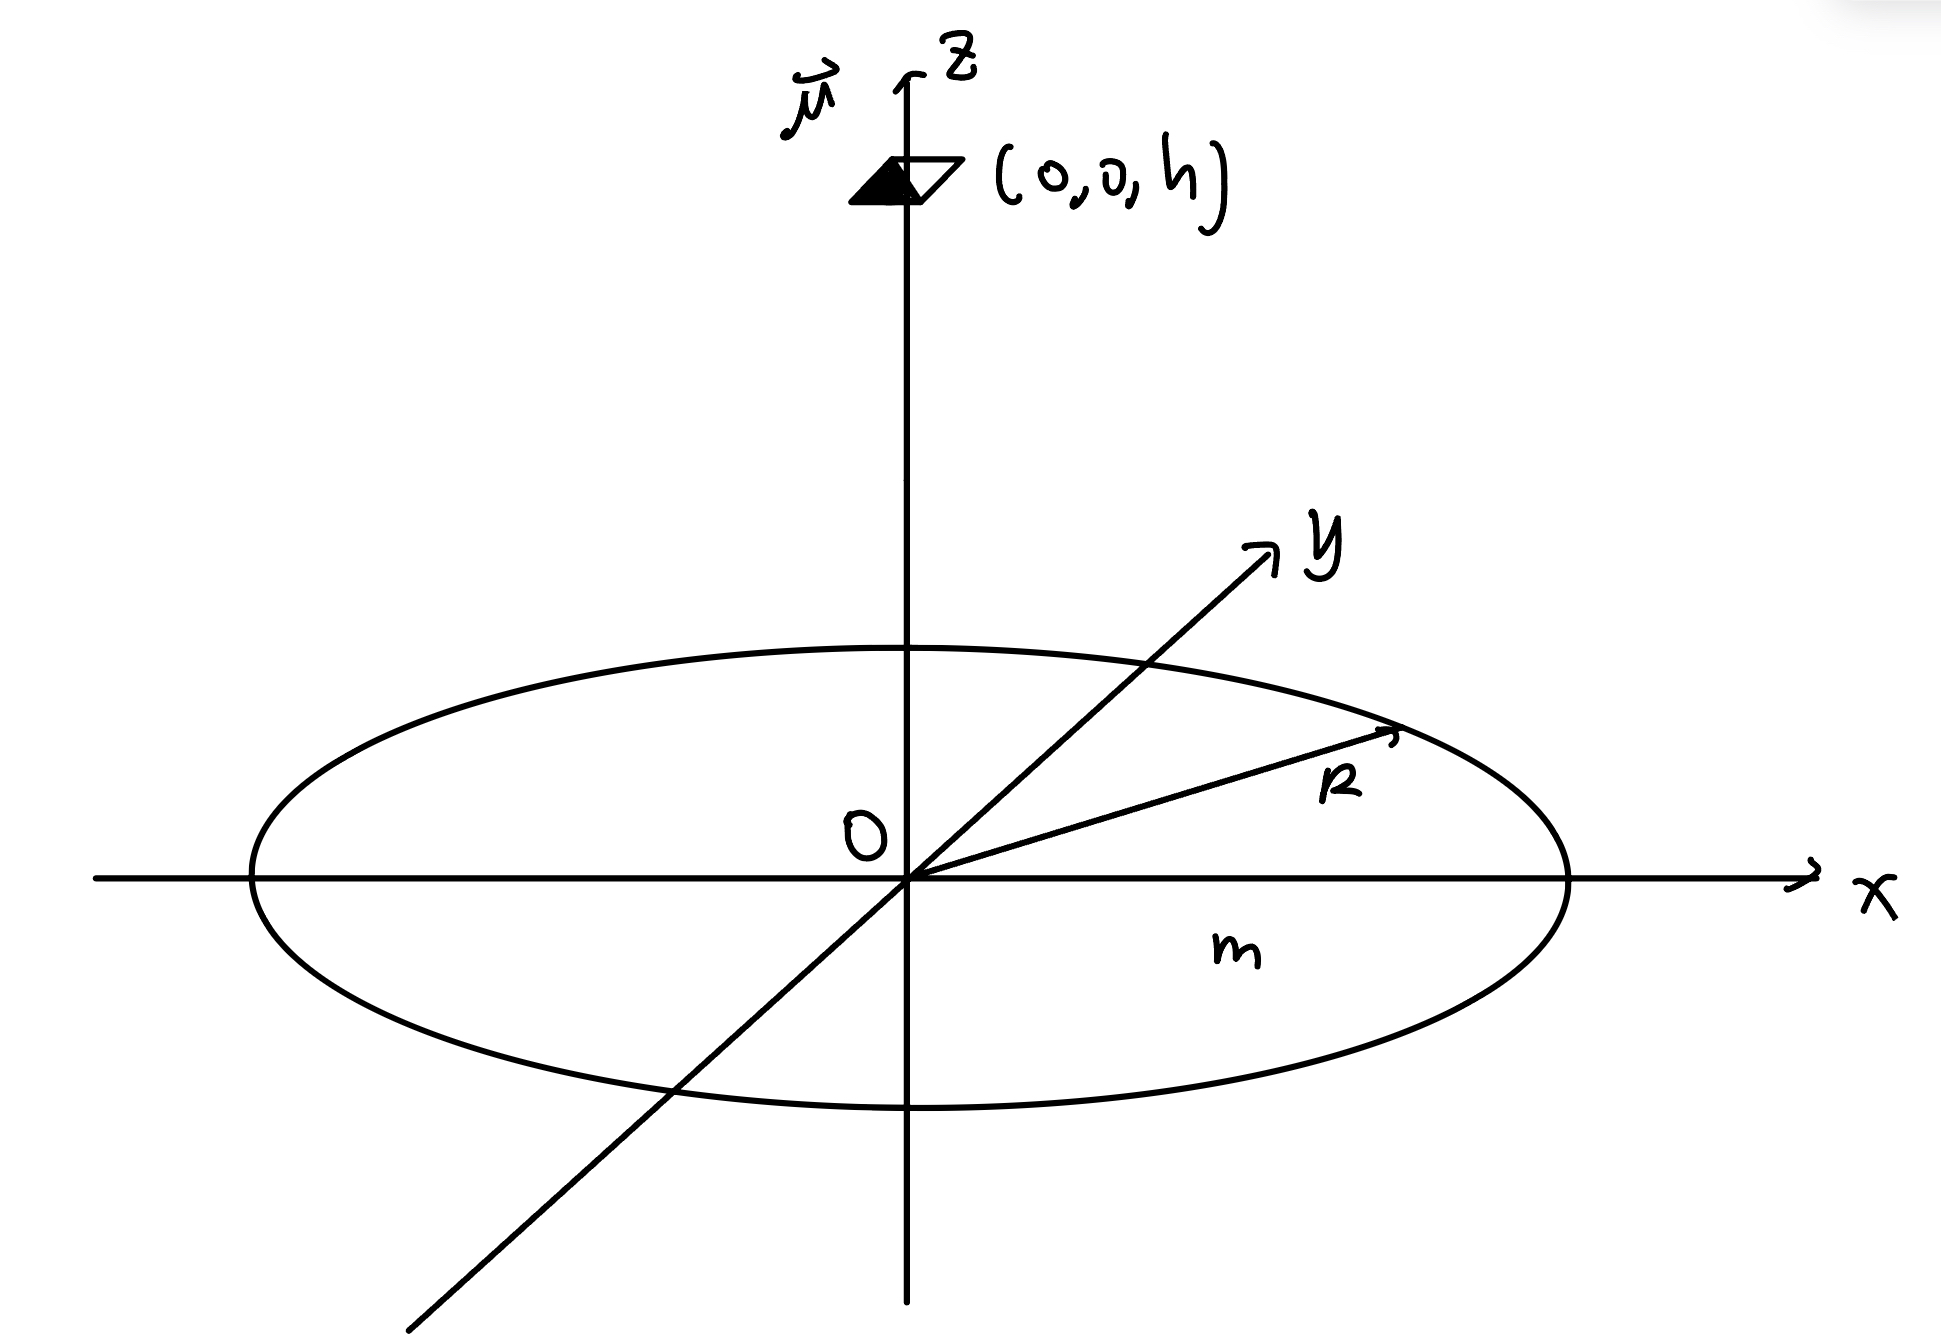
\includegraphics[width=7cm]{img/6.1.jpeg}\\
	\vspace{-15pt}    % 对应高度2
	\vspace{-15pt}    % 对应高度3
\end{wrapfigure}
高二这次期中考考了一个有关于Arago圆盘的选择题,小H同学对J老师的解释不是很满意,于是他尝试自己着手计算一下。\par
将小磁针认为是一个磁偶极子,大小为$\mu$。下方$h$处有一个带电薄圆盘质量为$m$,半径为$R$,以$\omega$转动。
\begin{itemize}
    \item[(1)]现固定小磁针,将下方带电薄圆盘以$\Omega$恒定速度转动,求小磁针受到的力矩。
    \item[(2)]现释放小磁针,并解除下方维持带电薄圆盘匀速转动的力矩,求两者共速后的共同角速度$\Omega$.
\end{itemize}
补充:磁偶极子的场
\[
\vec{B}=\dfrac{\mu}{4\pi}\dfrac{(3(\vec{\mu}\cdot\hat{r})\hat{r}-\vec{\mu})}{|\vec{r}|^3}
\]

\[\]
(1)
\[
\vec{B }=\dfrac{\mu _{0}}{4\pi }\dfrac{3\left( \vec{\mu }\cdot \hat{r}\right) \hat{r}-\vec{\mu }}{r^{3}}
\tag{1}\]
\[
\begin{aligned}
&\vec{F}=q\vec{v}\times\vec{B}=q(\vec{\omega}\times\vec{\rho})\times\vec{B}\\
&=q\left[\left(\vec{\omega}\cdot\vec{B}\right)\vec{\rho}-\left(\vec{\omega}\cdot\vec{\rho}\right)\vec{B}\right]\\
&=q\left(\vec{\omega}\cdot\vec{B}\right)\vec{\rho}
\end{aligned}
\tag{2}\]
\[
\vec{\mu}=\mu\left(\cos \varphi,\sin \varphi,0\right)
\tag{3}\]
\[
\vec{r}=\left(\rho\cos\theta,\rho\sin\theta,-h\right)
\tag{4}\]
\[
B_z=\frac{\mu_0}{4\pi}\frac{3\mu\rho\cos(\varphi-\theta)(-h)}{r^5}
\tag{5}\]
(2)认为$\vec{E}=\vec{v}\times\vec{B}$为等效电场
\[
\begin{aligned}
&\vec{j}=\sigma\vec{E}=\sigma(\vec{\omega}\cdot\vec{B})\vec{r}   \\
&=\dfrac{\sigma\mu_0\omega3\mu\rho\cos(\varphi-\theta)(-5)}{u\pi r^5}(\rho \cos\theta,\rho\sin \rho,0)
\end{aligned}
\tag{6}\]
\[
\vec{B}=\frac{\mu_0}{4\pi}\int\dfrac{\vec{j}\cdot\mathrm{d}V\times(-\vec{r})}{r^3}
\tag{7}\]
积分得
\[
\vec{B}=\left(\dfrac{\mu_0}{4\pi}\right)^2\frac{3\sigma\omega\mu h^2\pi}{2}\left[\dfrac{1}{2}\left(\dfrac{1}{h^4}-\dfrac{1}{\left(R^2+h^2\right)^2}\right)+\dfrac{h^2}{3}\left(-\dfrac{1}{h^6}+\dfrac{1}{\left(R^2+h^2\right)^3}\right)\right](-\sin\varphi \hat{x}+\cos \varphi \hat{y})
\tag{8}\]
令
\[
k=\left(\dfrac{\mu_0}{4\pi}\right)^2\frac{3\sigma\mu h^2\pi}{2}\left[\dfrac{1}{2}\left(\dfrac{1}{h^4}-\dfrac{1}{\left(R^2+h^2\right)^2}\right)+\dfrac{h^2}{3}\left(-\dfrac{1}{h^6}+\dfrac{1}{\left(R^2+h^2\right)^3}\right)\right]
\tag{9}\]
由力矩公式
\[
\vec{M}=\vec{v}\times\vec{B}=k\mu\omega\hat{z}
\tag{10}\]
\textbf{评分标准:}\par
共$40$ 分\par
(1)共$10$分 $(1),(2),(3),(4),(5)$各$2$分\par
(2)共$30$分 $(6),(7),(8),(9),(10)$各$6$分\par

\section*{第七题、“简单力学题”(50分)}
\begin{wrapfigure}{r}{4cm}
	\vspace{-15pt}    % 对应高度1
	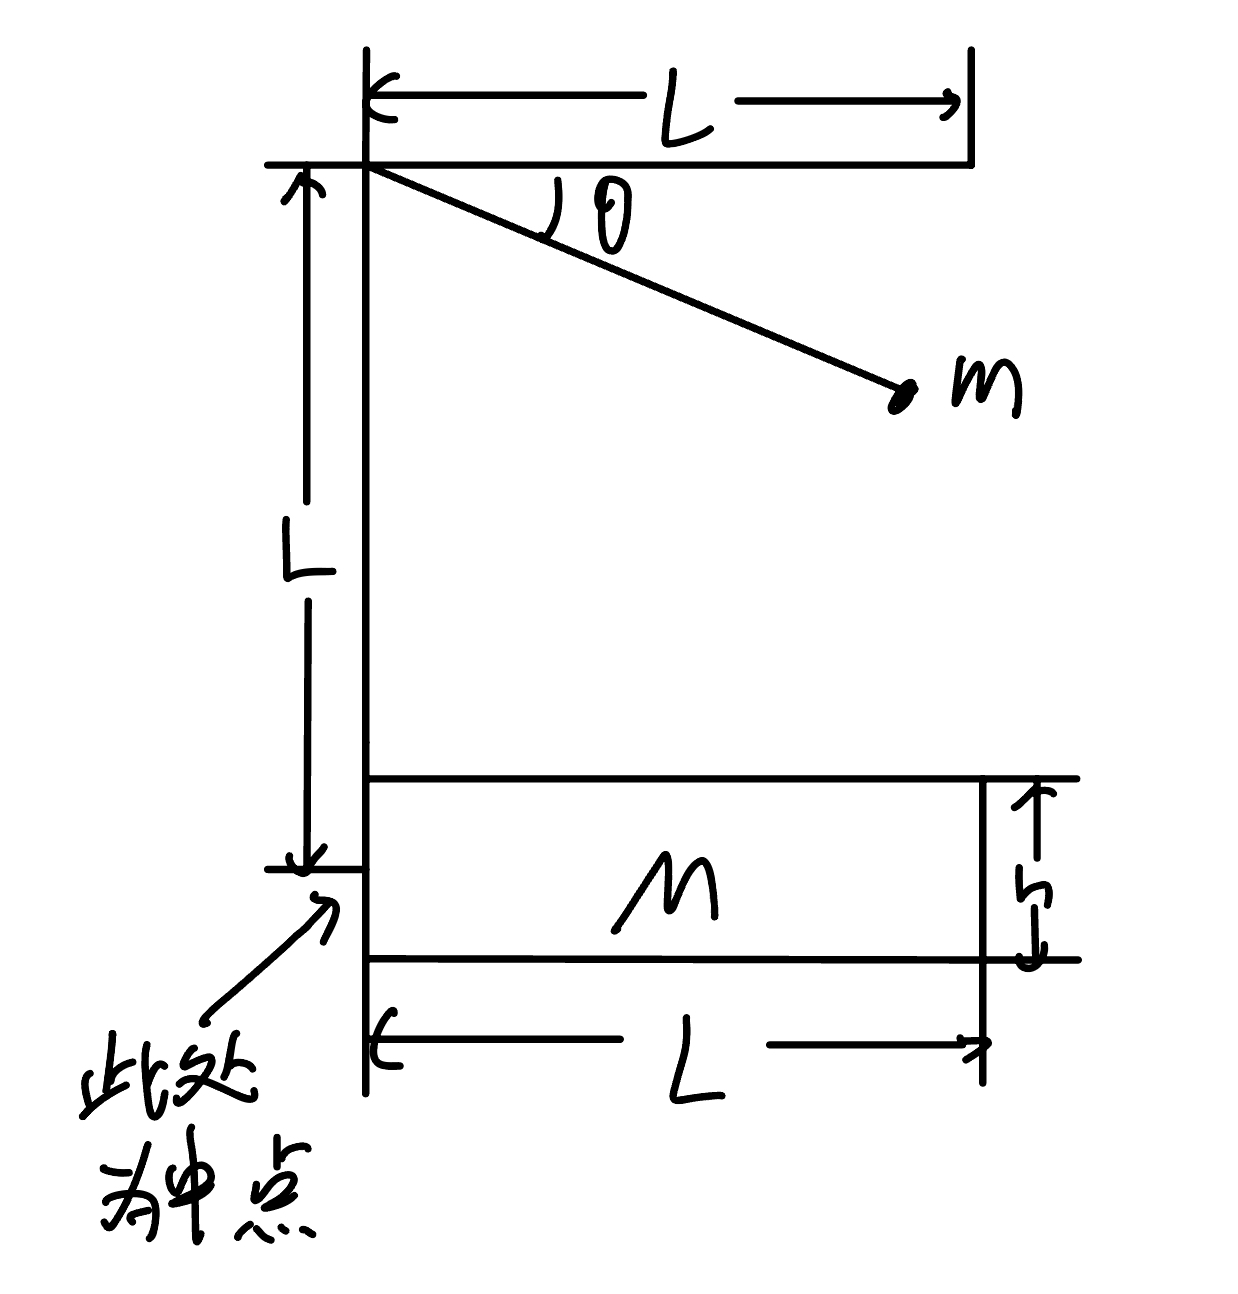
\includegraphics[width=4cm]{img/7.1.jpeg}\\
	\vspace{-15pt}    % 对应高度2
	\vspace{-15pt}    % 对应高度3
\end{wrapfigure}
光滑水平面上有一木块,匀质质量为$M$,在左端中间固定有一档板,其上有一绳,一侧系有一质量为$m$得质点。其中各参数如图所示,初态均静止,细绳水平释放质点。
试就$\frac{M}{m}=1,\frac{1}{2}$时,求木块右侧是否会离开地面。若会,其第一次离开时的$\theta$ .

\[\]
由能动量定理
\[
\begin{cases}
    Mv=m\left( L\dot{\theta} \sin \theta -v\right) \\
    \dfrac{1}{2}mv^{2}+\dfrac{1}{2}m\left( 2\dot{\theta} \sin \theta -v\right) ^{2}+\dfrac{1}{2}m\left( L\dot{\theta}\cos \theta \right) ^{2}=mgL\sin \theta 
\end{cases}
\tag{1}\]
解得
\[
\dot{\theta} =\sqrt{\dfrac{2\left( M+m\right) g\sin \theta }{L\left( M+m\cos^2\theta \right) }}
\tag{2}\]
\[
v=\dfrac{mL\sin \theta }{M+m}\sqrt{\dfrac{2\left( M+m\right) g\sin \theta }{L\left( M+m\cos ^{2}\theta \right) }}
\tag{3}\]
\[
a=\dfrac{\mathrm{d}v}{\mathrm{d}t}=\dfrac{\mathrm{d}v}{\mathrm{d}\theta }\dot{\theta}=\dfrac{m\left[ \left( 3M+2m\right) \sin \theta \cos \theta +m\sin \theta \cos ^{3}\theta \right] }{\left( M+m\cos^{2}\theta \right) ^{2}}g
\tag{4}\]
% \par
% \begin{wrapfigure}{r}{7cm}
% 	\vspace{-5pt}    % 对应高度1
% 	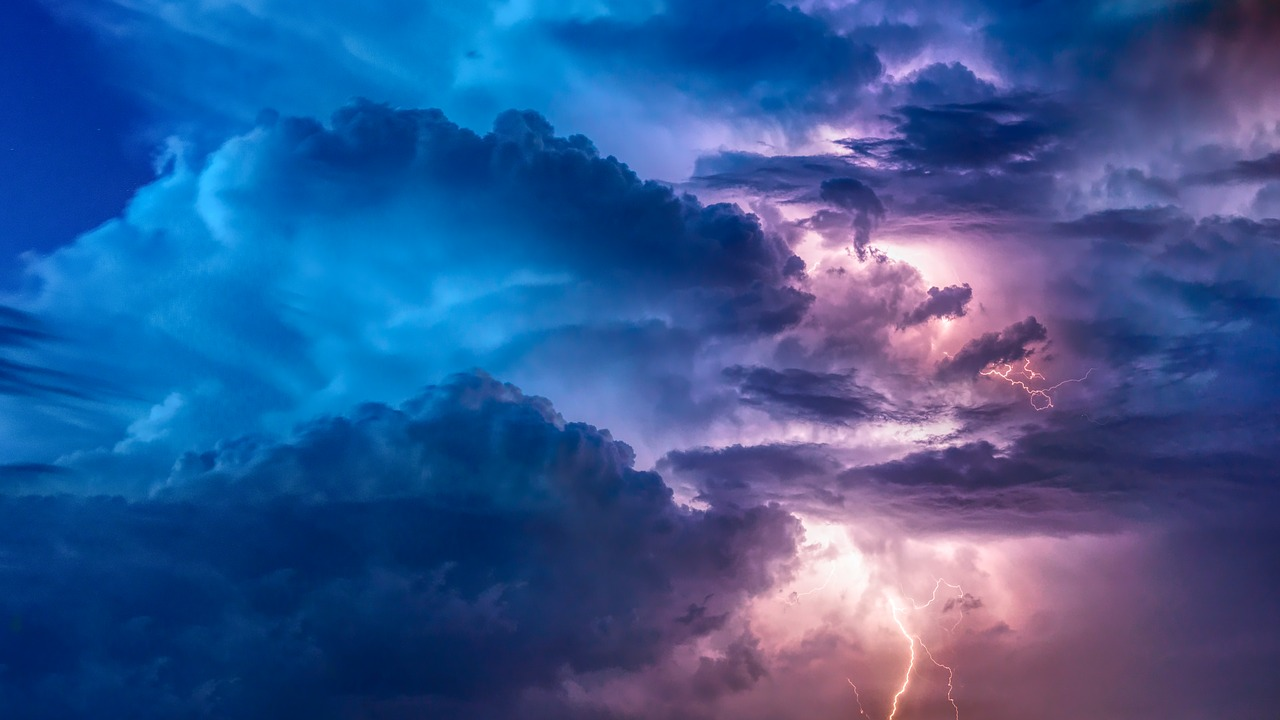
\includegraphics[width=7cm]{img/2.jpeg}\\
% 	\vspace{-5pt}    % 对应高度2
% 	\caption{}
% 	\vspace{-5pt}    % 对应高度3
% \end{wrapfigure}
在木块系中($F$为绳子拉力)
\[
F\cos \theta=Ma
\tag{5}\]
考虑临界情况
\[
 -Mg\dfrac{L}{2}-Ma\dfrac{h}{2}+F\cos \theta \left(L+\dfrac{h}{2}\right) -F\sin \theta L\geq 0
\tag{6}\]
化简得
\[
a\geq\dfrac{g}{2(1-\tan\theta)}
\tag{7}\]
即
\[
\dfrac{2m\left[ \left( 3M+2m\right) \left( \sin \theta \cos \theta \right) +msin\theta \cos ^{3}\theta \right] \left( 1-\tan \theta \right) }{\left( M+m\cos ^{2}\theta \right) ^{2}}\geq 1
\tag{8}\]
令$\frac{M}{m}= k$,$\tan\theta= t$
\[
\alpha =\dfrac{2\left[ \left( 3k+2\right) \left( 1+t^{2}\right) t+t\right] \left( 1-t\right) }{\left[ k\left( 1+t^{2}\right) +1\right] ^{2}}\geq 1
\tag{9}\]
对(6)左式求导取极值
\[
\left[ k\left( 1+t^{2}\right) +1\right] \left\{ \left[ \left( 3k+2\right) \left( 1+3t^{2}\right) +1\right] \left( 1-t\right) -\left[ \left( 3k+2\right) \left( 1+t^{2}\right) t+t\right] \right\} =4kt\left( 1-t\right) \left[ \left( 3k+2\right) \left( 1+t^{2}\right) t+t\right] 
\tag{10}\]
\[
\left( 3k^{2}+2k\right) t^{4}+\left( 6k^{2}+14k+8\right) t^{3}-\left( 6k+b\right) t^{2}+\left( 6k^{2}+12k+6\right) t-\left( 3k^{2}+6k+3\right) =0
\tag{11}\]
\[
代入k=1解得t=0.4765453307
\tag{12}
\]
\[
代入(11)解得\alpha=0.7177259631<1,故不会翻起
\tag{13}
\]
\[
代入k=\frac{1}{2}解得t=0.5043814407
\tag{14}
\]
\[
代入(11)解得\alpha=1.017831264>1,故会翻起,可得\theta=23.688^{\circ}
\tag{15}
\]
\textbf{评分标准:}\par
共$50$ 分\par
$(1),(2),(3),(4),(5),(7),(8),(9),(10),(11)$各$3$分,$(12),(13),(14),(15)$各$5$分

\end{document}